\chapter{图片和表格}
\section{插入图片}
使用如下代码
\begin{verbatim}
	\begin{figure}[H]
		\centering %居中
		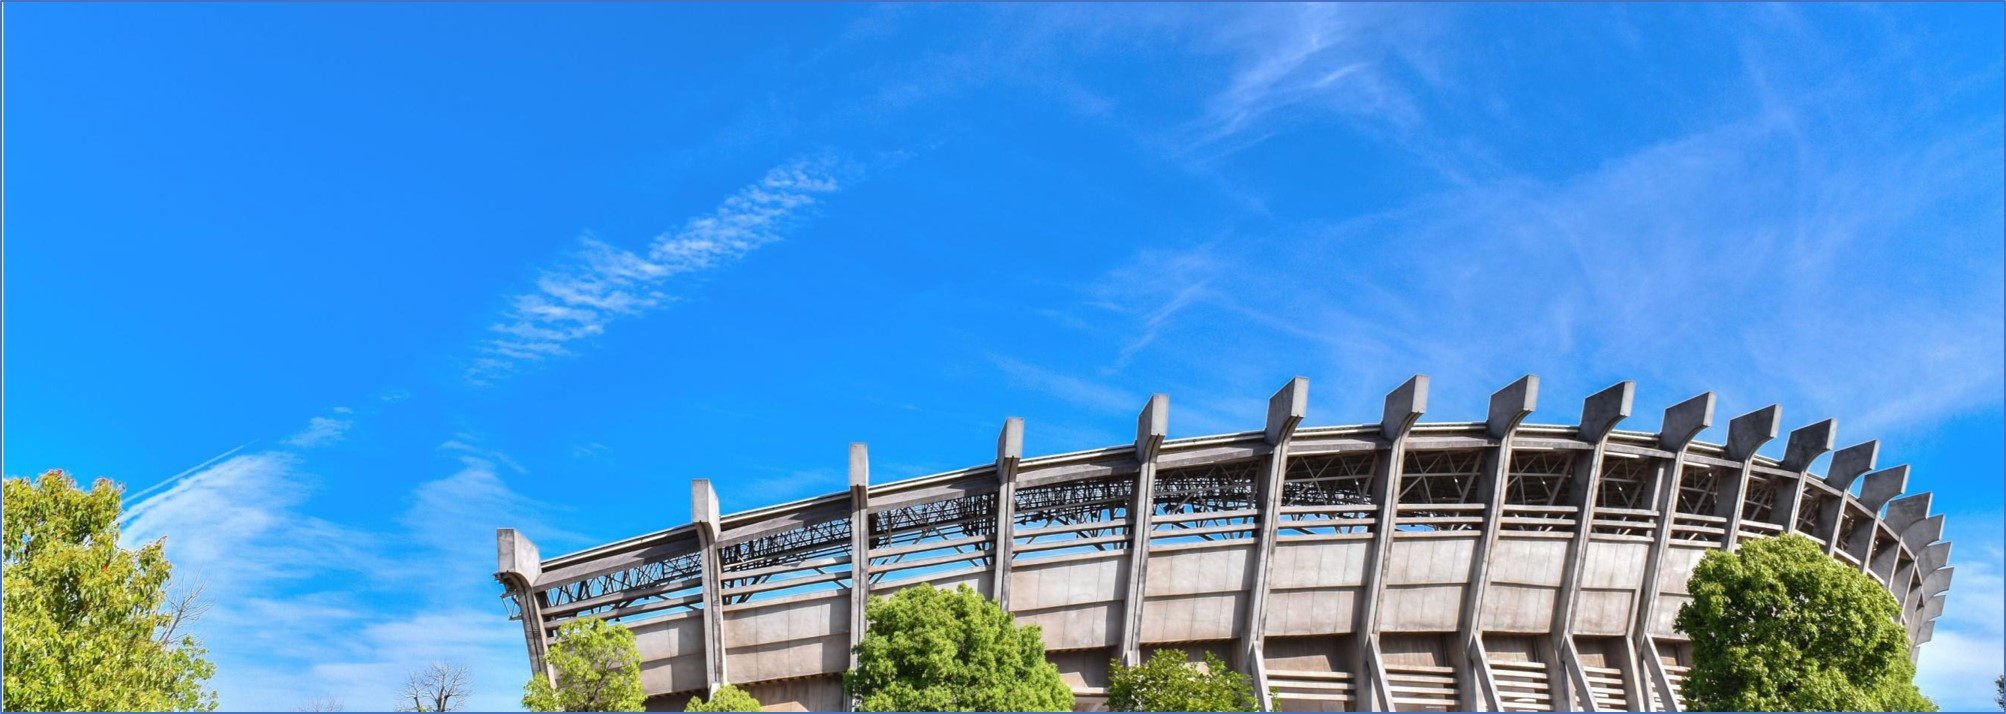
\includegraphics[width=0.8\linewidth]{figures/csu} %图片文件位置以及图片文件名
		\caption{中南大学} %图题
		\label{fig:csu} %图片的label,上下文中引用该图片的时候需要用到
	\end{figure}
\end{verbatim}
插入如图\ref{fig:csu}所示的图片
\begin{figure}[H]
	\centering %居中
	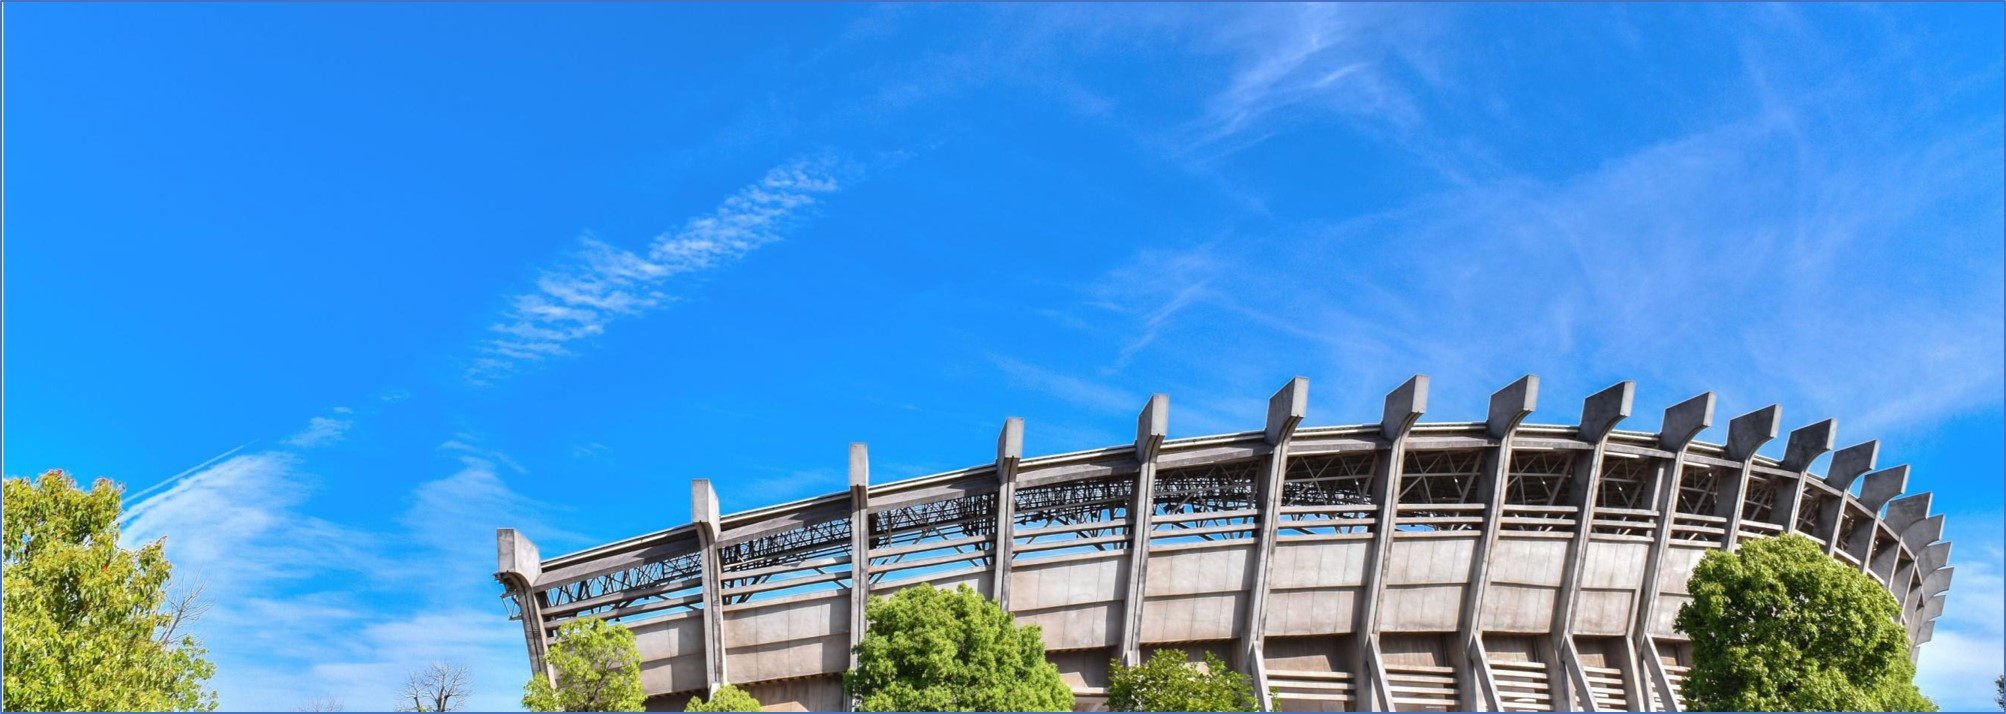
\includegraphics[width=0.8\linewidth]{figures/csu} %文件名
	\caption{中南大学} %图题
	\label{fig:csu} %图片的label,上下文中引用该图片的时候需要用到
\end{figure}

的图片。引用图片编号使用\verb|\ref{图片label}|。


\section{插入表格}
使用如下代码,
\begin{verbatim}
\begin{table}[H]
	\centering
	\topcaption{成绩单}\label{tab:scores}
	\begin{tabular}{ccc}
		\toprule % toprule 三线表的顶线
		姓名 & 高等数学 & 线性代数 \\
		\midrule % midrule 三线表的中线
		张三 & 100 & 100 \\
		李四 & 101 & 101 \\
		\bottomrule % bottomrule 三线表的底线
	\end{tabular}
\end{table}
\end{verbatim}
可以得到如表\ref{tab:scores}所示的表格
%三线表,toprule和bottom分别是顶线和底线,midrule是中间的线
%\topcaption是我重新定义的表题命令,目的是减小表题与表格间距离,见dissertation.tex文件105-110行
\begin{table}[H]
\centering
\topcaption{成绩单}\label{tab:scores}
\begin{tabular}{ccc}
	\toprule 
	姓名 & 高等数学 & 线性代数 \\
	\midrule
	张三 & 100 & 100 \\
	李四 & 101 & 101 \\
	\bottomrule
\end{tabular}
\end{table}
